
%(BEGIN_QUESTION)
% Copyright 2012, Tony R. Kuphaldt, released under the Creative Commons Attribution License (v 1.0)
% This means you may do almost anything with this work of mine, so long as you give me proper credit

Dette solcelledrevne pumpesystemet har et problem.  Pumpemotoren skal slå seg på etter en tidsplan satt av tidsbryteren, men pumpen starter aldri selv om solen skinner fullt på de strømproduserende solpanelene.  Hvert panel gir 22 volt i åpen krets (dvs. uten last) og 15 volt når det driver pumpemotoren:

$$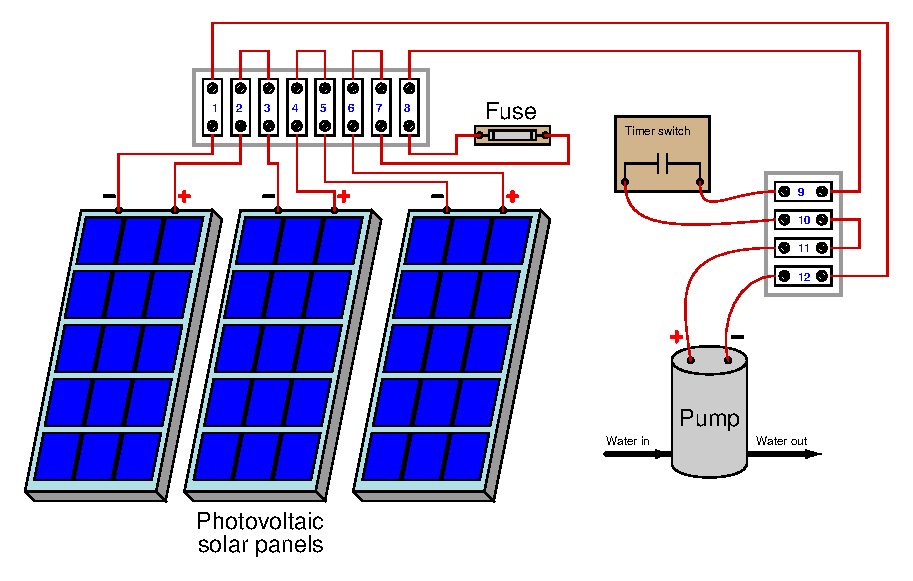
\includegraphics[width=15.5cm]{i01141x01.eps}$$

Et DC-voltmeter koblet mellom terminal 9 og 12 viser 0 volt når solen skinner sterkt og tidsbryteren skal stå i ``på''-stilling for å kjøre pumpen.  Vurder sannsynligheten for hver oppgitt feil i denne kretsen.  Vurder én feil om gangen (dvs. ingen sammenfallende feil), og avgjør om hver feil alene kan forklare {\it alle} målinger og symptomer i kretsen.

% No blank lines allowed between lines of an \halign structure!
% I use comments (%) instead, so that TeX doesn't choke.

$$\vbox{\offinterlineskip
\halign{\strut
\vrule \quad\hfil # \ \hfil & 
\vrule \quad\hfil # \ \hfil & 
\vrule \quad\hfil # \ \hfil \vrule \cr
\noalign{\hrule}
%
% First row
{\bf Feil} & {\bf Mulig} & {\bf Umulig} \cr
%
\noalign{\hrule}
%
% Another row
Ledning mellom terminal 8 og 9 har åpen feil &  &  \cr
%
\noalign{\hrule}
%
% Another row
Ledning mellom terminal 1 og 12 har åpen feil &  &  \cr
%
\noalign{\hrule}
%
% Another row
Ledning mellom terminal 5 og solpanel har åpen feil &  &  \cr
%
\noalign{\hrule}
%
% Another row
Ledning mellom terminal 10 og 11 har åpen feil &  &  \cr
%
\noalign{\hrule}
%
% Another row
Tidsbryter har kortslutningsfeil &  &  \cr
%
\noalign{\hrule}
%
% Another row
Tidsbryter har åpen feil &  &  \cr
%
\noalign{\hrule}
%
% Another row
Sikring er gått (åpen) &  &  \cr
%
\noalign{\hrule}
%
% Another row
Pumpemotor har åpen feil &  &  \cr
%
\noalign{\hrule}
} % End of \halign 
}$$ % End of \vbox

\underbar{file i01141}
%(END_QUESTION)





%(BEGIN_ANSWER)

% No blank lines allowed between lines of an \halign structure!
% I use comments (%) instead, so that TeX doesn't choke.

$$\vbox{\offinterlineskip
\halign{\strut
\vrule \quad\hfil # \ \hfil & 
\vrule \quad\hfil # \ \hfil & 
\vrule \quad\hfil # \ \hfil \vrule \cr
\noalign{\hrule}
%
% First row
{\bf Feil} & {\bf Mulig} & {\bf Umulig} \cr
%
\noalign{\hrule}
%
% Another row
Ledning mellom terminal 8 og 9 har åpen feil & $\surd$ &  \cr
%
\noalign{\hrule}
%
% Another row
Ledning mellom terminal 1 og 12 har åpen feil & $\surd$ &  \cr
%
\noalign{\hrule}
%
% Another row
Ledning mellom terminal 5 og solpanel har åpen feil & $\surd$ &  \cr
%
\noalign{\hrule}
%
% Another row
Ledning mellom terminal 10 og 11 har åpen feil &  & $\surd$ \cr
%
\noalign{\hrule}
%
% Another row
Tidsbryter har kortslutningsfeil &  & $\surd$ \cr
%
\noalign{\hrule}
%
% Another row
Tidsbryter har åpen feil &  & $\surd$ \cr
%
\noalign{\hrule}
%
% Another row
Sikring er gått (åpen) & $\surd$ &  \cr
%
\noalign{\hrule}
%
% Another row
Pumpemotor har åpen feil &  & $\surd$ \cr
%
\noalign{\hrule}
} % End of \halign 
}$$ % End of \vbox


%(END_ANSWER)





%(BEGIN_NOTES)

{\bf Denne oppgaven er kun ment for prøver/eksamen, ikke arbeidsark!}.

%(END_NOTES)


